\documentclass[12pt,a4j,titlepage]{ltjsarticle}
\usepackage{semi}
\setcounter{tocdepth}{3}

\begin{document}
\begin{titlepage}
  \centering
    \vspace*{40truept}
    {\LARGE 2022年度 卒業論文}
    
    \vspace*{75truept}
    
    {\Huge 娯楽ゲームの教育的活用を推進する}
\vspace*{10truept}

    {\Huge Webサイトによる印象変化の調査}%論文タイトル

    \vspace{85truept}
    
    {\LARGE 指導教員 須田 宇宙 准教授}
    
    \vspace{60truept}
    
    {\LARGE 千葉工業大学 情報ネットワーク学科}
    
    \vspace{15truept}
    
    {\LARGE 須田研究室}
    
    \vspace{70truept}
    
    {\LARGE 1732008 氏名 五十嵐 美結 } % 氏名は消さない 学生番号 氏名 名前

    \vspace{70truept}
    
  \begin{flushright}

    \LARGE {提出日 2023年1月17日}
  
  \end{flushright}
\end{titlepage}
\date{}



\tableofcontents
\listoftables
\listoffigures
\clearpage
%1章
\section{緒言}\label{緒言}
%1章には,背景・問題点・目的を順番に書く.
%背景は,広く一般的な事柄を書いて,読む人に同意を抱かせつつ問題点につなぐ.
%問題点では,「〜という問題点がある」などのように,「問題」または「問題点」と言う単語を用いて,目的につなぐ.
%目的では,「そこで本研究では」から始めて,「〜を目的とする」で締める.
%以下は過去の卒業研究最終審査用の梗概の抜粋である.

%背景
近年,アクティブ・ラーニングとして授業活動にゲーミフィケーションといわれるゲームの娯楽性要素や,学習要素を盛り込んだシミュレーション等のゲーム(シリアスゲーム)を導入する動きが活発になってきている.
ゲーミフィケーションは楽しさ,目的意識,達成感の充実といったゲームの主要な要素を取り入れることによって授業への参加意欲や充実感の向上のために活用されている.
シリアスゲームはデジタルゲームの一種で主にコンピュータやタブレットなどを使用し,教育・医療・環境といった社会問題の解決を目的として,英語やプログラミング分野では実際に教育現場で活用されている.

%問題点
一方でデジタルゲームのうち、学習目的でない娯楽要素の多いゲームはゲーム依存症やゲーム脳等のイメージがあり、教育的なメリットや学習機会があることは周知されておらず自宅での学習の妨げになる等の悪い印象が広まってしまっている。
またこの問題のよって保護者からプレイの制限をされることで、ゲームから得られる学習機会の損失になるという問題点がある。

そこで本研究では,学習を主目的としないデジタル娯楽ゲームの印象の改善とそれらの持つ教育的効果の周知を図るために,様々な娯楽ゲームの持つ教育的なメリットをタグ付けしたWebサイトの開発をし,それにより娯楽ゲームに教育効果や学習機会があることを理解したかを保護者へのアンケート調査を行い評価することを目的とする.
%2章
\section{ゲームについて}
\subsection{教育に活用されるゲームと娯楽ゲーム}
本稿で扱うゲームの種類は家庭用ゲーム機やパソコン,タブレット,スマートフォン等でプレイするデジタルゲームである.
またそのゲームは大まかに教育や学習目的のものと娯楽向けのゲームに分けることができる.

\subsubsection{教育に活用されるゲーム}\label{教育ゲーム}
\ref{緒言}で記述したシリアスゲームは学習や社会問題の解決のための専門的に開発されたゲームであり,海外の学校等の教育現場でギガタブ等のコンピュータを利用し導入されている.
例としてKONAMIが国連世界食料計画(WFP)と協力し発売した「Food Force」というゲームがあり,これは世界の飢餓撲滅のための食糧支援の活動が学べるものである.
プレイヤーはWFPの一員となり飢餓地域に食糧を届けるために物資を確保し輸送,緊急事態にも対処しながら実際に行われている支援をゲームを通して学び,考えを深めることができる.

シリアスゲームの他にも英語やプログラミングなどの学習のためのゲームや算数・数学の図形をシミュレーションするゲームなどがある.

\subsubsection{娯楽ゲーム}
本研究で主に扱っている娯楽ゲームは\ref{教育ゲーム}で述べたような学習が主目的のゲームとは違い,楽しさや達成感,感動,ストレス解消などを得ることが主目的のゲームで娯楽向けのものを指す.

\subsection{ゲームに関する課題}
インターネットやゲーム機器の技術発達に伴い使用者の低年齢化が進み,日常生活の一部や学習,娯楽に使用されるようになった.その反面,過剰な利用や有害な事物に触れることが増えている.
ゲームに関しては過剰利用によるゲーム依存やゲーム脳の問題があり,ニュース等で取り上げられるなどして問題視されている.

\subsubsection{ゲーム依存・ゲーム脳}


\subsubsection{香川県ネット・ゲーム依存症対策条例}

%3章
\section{アンケート調査}\label{アンケート調査}
\ref{Webサイトについて}章で述べるサイトを対象者が閲覧した後の娯楽ゲームの教育的なメリットへの理解とイメージの変化を調査するためにアンケートを行った.
\subsection{調査概要}
調査対象である小中学生の子を持つ保護者10人に調査を行った.対象者の情報については表\ref{}の通りで,子の年齢やゲーム機の所持状況の他に回答者や子の週にゲームをプレイする頻度や好き嫌い,回答者の子供の頃のゲームプレイの頻度を収集した.

\begin{table}[h]
 \caption{対象者の情報}
 \label{table:anque}
 \small
 \centering
  \begin{tabular}{lrrrrrrrr}
  \hline
   子の年齢 & 未就学児 & 小学1,2年 & 3,4年 & 5,6年 & 中学1年 & 2年 & 3年 & 高校以上\\
   (人)& 2 & 3 & 2 & 4 & 3 & 1 & 2 & 0\\
   \hline
  \end{tabular}
\end{table}

\begin{table}[h]
 \caption{ゲーム機器の有無}
 \label{table:anque}
 \small
 \centering
  \begin{tabular}{rrrrr}
  \hline
  家庭用ゲーム機 & スマートフォン & PC & ギガタブ & 持っていない\\
   \hline
  \end{tabular}
\end{table}

\subsection{調査項目}

\begin{table}[h]
 \caption{アンケート}
 \label{table:anque}
 \small
 \centering
  \begin{tabular}{l}
  \hline
  子に与える影響について \\
   \hline \hline
   ⅰ.勉強面 \\
   ⅱ.友人関係,コミュニケーション\\
   ⅲ.感性\\
   ⅳ.知識,教養 \\
   ⅴ.時間管理   \\
   ⅵ.健康面 \\
   ⅶ.読書・スポーツ等他の趣味とのメリットの比較 \\
   \hline
  \end{tabular}
\end{table}

%4章
\section{Webサイトについて}\label{Webサイトについて}
\subsection{概要}
WebサイトはHTMLとCSSを使用して作成し,ツールとしてBootstrapを用いた.トップページに教育的メリットのタグ,教科,ゲーム一覧のボタンを設置し関連づいたゲームが表示されるようにした.構成の詳細については以下の通りである.
\subsection{ゲームの種類}
掲載したゲームは対象である小・中学生の年齢を加味し,Nintendo Switchのソフトとスマートフォンでプレイできるゲームを12個に絞った.また年齢に沿ったゲームの紹介を行う為,対象年齢を全年齢のもの9個と一部オンラインショップやバトルシーンがあり12・15歳以上になっているもの3個を掲載した.ゲーム一覧は以下の図\ref{fig:ゲーム一覧}の通りである.
教育メリットと教科の説明等

\subsection{ゲーム記事}

\vspace{1zh}
\begin{figure}[h]
\begin{center}
 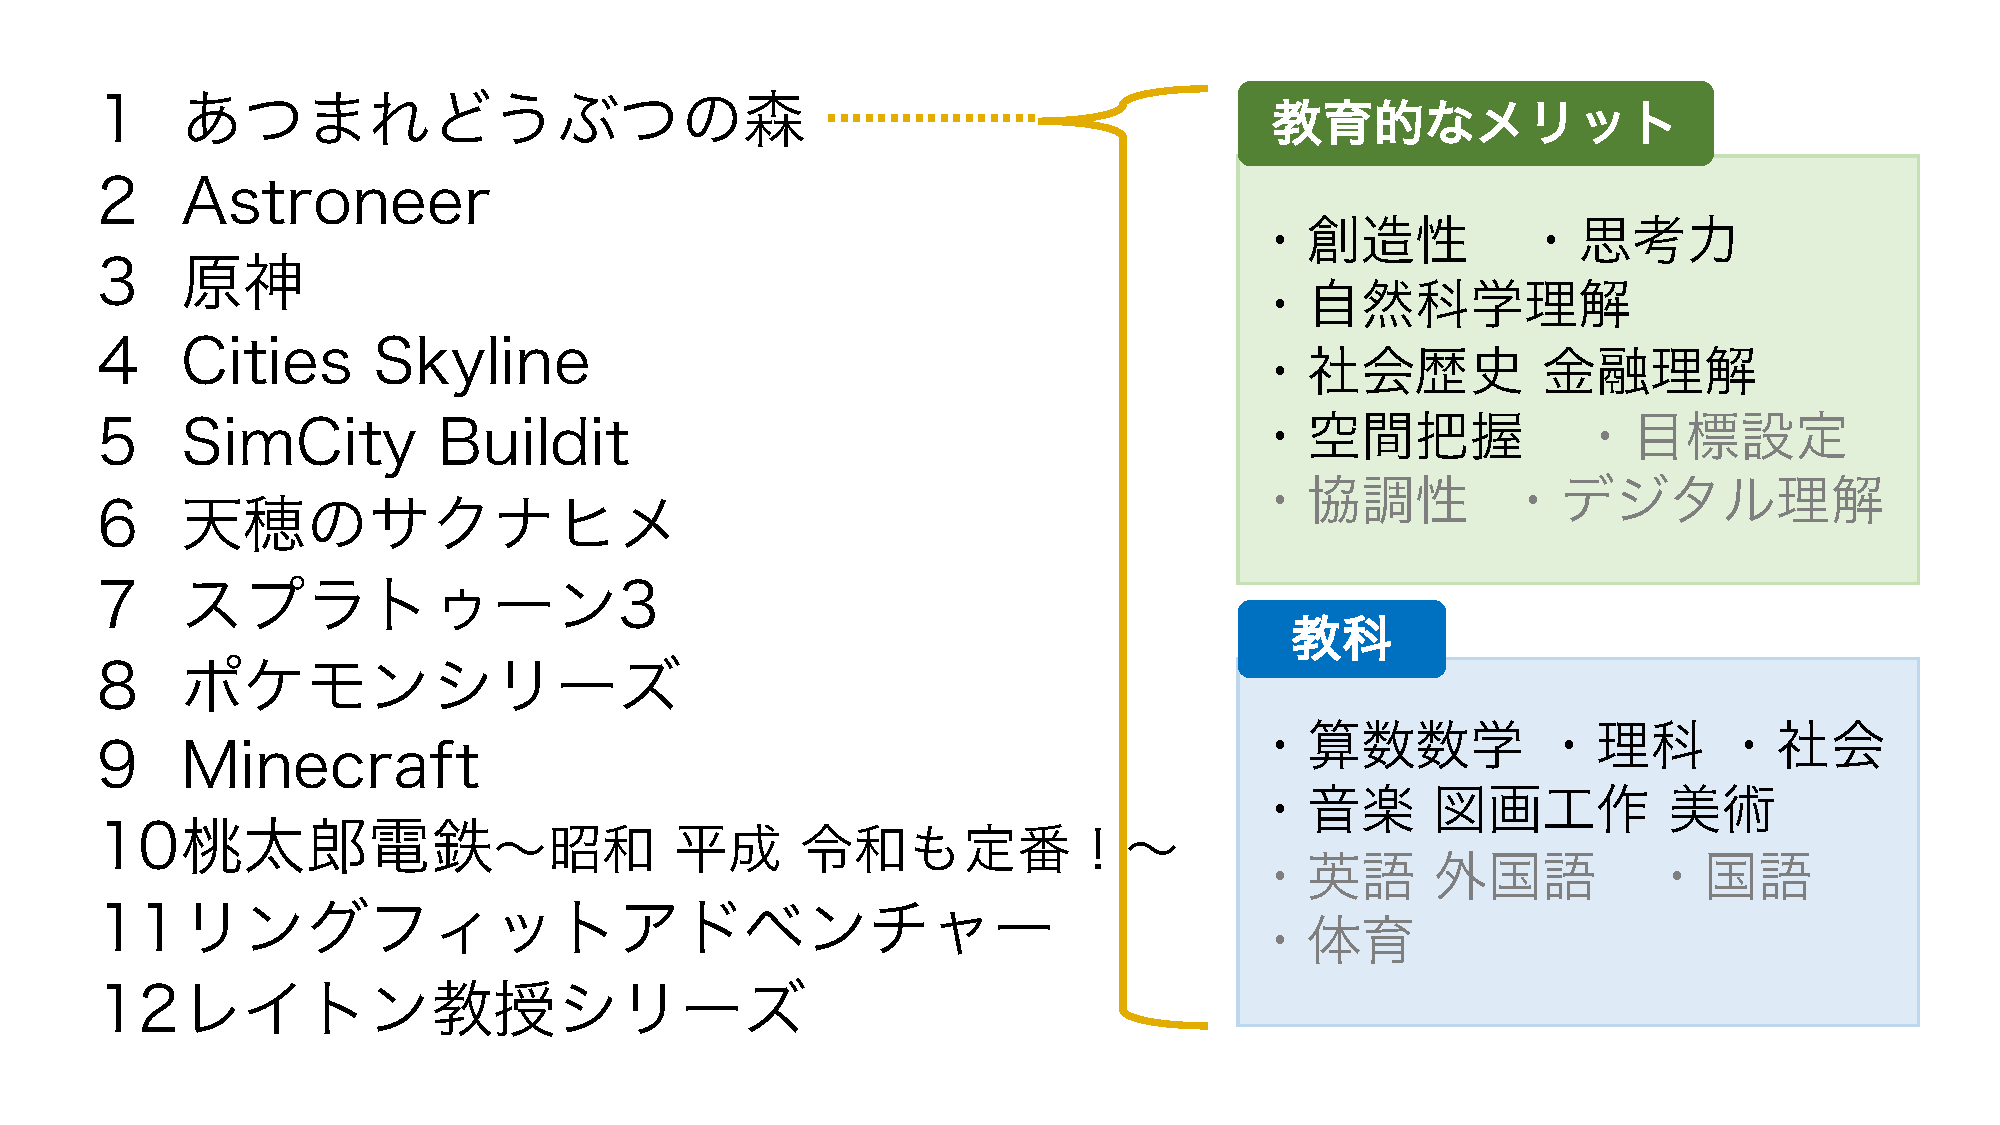
\includegraphics[clip,width=95mm,height=55mm]{games.pdf}
\end{center}
 \caption{ゲーム一覧とあつまれどうぶつの森のタグ付け例}
 \label{fig:ゲーム一覧}
\end{figure}

%5章
\section{評価}
\subsection{概要}
\subsection{アンケートの評価}
%6章
\section{結言}

\section{謝辞}

\begin{thebibliography}{99}
\bibitem{gameanq} ASMARQ : ``ゲームと子どもに関するアンケート調査'', \url{https://www.asmarq.co.jp/data/mr201409game/}, 2022/8/19参照
\bibitem{tvgame} 坂元 章 : ``21世紀はテレビゲーミング社会 ―娯楽主導から有効利用ヘ―'', 特定非営利活動法人日本シミュレーション&ゲーミング学会, 2000年 10 巻 1 号 p. 4-13, 2000.
\end{thebibliography}

\end{document}
